\newpage
\section{Interdependencia y ganancias derivadas del comercio} La interdependencia entre productores debe entenderse como una forma de producción mas eficiente, con una mayor variedad de productos disponibles para el consumidor. Por lo que se parte del comercio implica un aumento de la prosperidad y eficiencia entre las partes. 
\\
Se puede representar via FPP la produccion sin comercio de una persona o pais. A su vez, la apertura al comercio, siempre muestra posibilidades de consumo antes inalcanzables. 
\subsection{Ventajas} Cuando un productor puede generar el mismo producto con una menor cantidad de factores se dice que tiene una ventaja absoluta.
\\
Ventaja relativa acorde a un productor que tiene un coste de oportunidad mas bajo(comparando costes entre productores )
\subsection{Importaciones} Productos producidos fuera del territorio nacional,en dondé se tiene una desventaja relativa o absoluta en la producción. Consumidos al interior del territorio. 
\subsection{Exportaciones} Productos producidos fentro del territorio nacional, en dondé se tiene una ventaja absoluta o relativa. Consumidos al fuera del territorio.
\\
El comercio siempre generara interdependencia entre actores de un mercado.

\begin{figure}[h]
	\centering
   \begin{subfigure}[h]{0.2\textwidth}
	\begin{tikzpicture}[scale=0.7]
\draw (0,5.1) node [left] {$Y$} -- (0,0) node [below left] {$0$} -- (4,0) node [below] {$X$};
\draw [blue](0,4) to [out=-15, in=120] (1.9,1.8) to [out=-70, in=95] (2,0);
\draw (0,2.1) to [out=-15, in=120] (1.8,1) to [out=-60, in=95] (2,0);

\end{tikzpicture}
		\caption{FPP Mejora en factor Y }
	\end{subfigure}
\begin{subfigure}[h]{0.2\textwidth}
	\begin{tikzpicture}[scale=0.7]
	\draw (0,5.1) node [left] {$Y$} -- (0,0) node [below left] {$0$} -- (4,0) node [below] {$X$};
	\draw[Red] (0,2.1) to [out=-15, in=120] (3,1.5) to [out=-60, in=95] (3.4,0);
	\draw (0,2.1) to [out=-15, in=120] (1.8,1) to [out=-60, in=95] (2,0);
	\end{tikzpicture}
	\caption{FPP Mejora en factor X }
\end{subfigure}
\begin{subfigure}[h]{0.2\textwidth}
	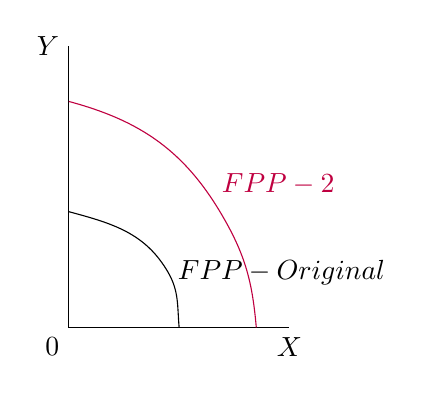
\begin{tikzpicture}[scale=0.7]
\draw (0,5.1) node [left] {$Y$} -- (0,0) node [below left] {$0$} -- (4,0) node [below] {$X$};
\draw[purple] (0,4.1) to [out=-15, in=120] (2.8,2) to [out=-60, in=95] (3.4,0);
\draw (0,2.1) to [out=-15, in=120] (1.8,1) to [out=-60, in=95] (2,0);
\node [right] at (1.8,1) {$FPP-Original$};	
\node [purple][right] at (2.6,2.6) {$FPP-2$};	
\end{tikzpicture}
	
	\caption{FPP Mejora en Ambos Factores}
\end{subfigure}	
\end{figure}
Existen distintas formas de mejoras en los factores a producir, ya sea con mejoras en la forma productiva (Tecnología)de un bien o de ambos. en ambos casos se logra alcanzar puntos que antes era inalcanzables para el productor.

